\section{Predicción lineal y síntesis de vocales}

\subsection{Generación de Tren de Impulsos}
Se crea la función $X = exciteV (N, N p)$ que representa el sonido de las cuerdas vocales mediante un tren
de impulsos, donde N es el largo de la señal en muestras y $Np$ el período en muestras. El código de la función generada se muestra a continuación:
\begin{lstlisting}[language = octave]
function y = exciteV(N,Np)
    y = zeros(1,N)
    for i = 1:N
        if mod(i-1,Np) == 0
            y(i) = 1;
    end
end
\end{lstlisting}

Posteriormente se genera un tren de impulsos de 100 Hz de duración $1~s$ muestreada a $8~kHz$, para luego escucharla y graficar su espectro en frecuencia. Lo anterior usando el script \texttt{p1\_1.m}, adjunto a la entrega.

La sección de código donde se genera la señal de tren de impulsos corresponde a:
\begin{lstlisting}[language = octave]
fs = 8000;
t =1;
f = 100;
T = fs/f;
y = exciteV(t*fs,T);
Y =   fft(y);
Ymod = abs(Y);
Ydb = 20*log10( 0.000000001 + Ymod(1:fs/2));  
plot([0:fs/2-1],  Ydb(1:fs/2));

\end{lstlisting}



El espectro obtenido para la señal generada se muestra en  la figura \ref{frec_tren}

\begin{figure}[H]
    \centering
    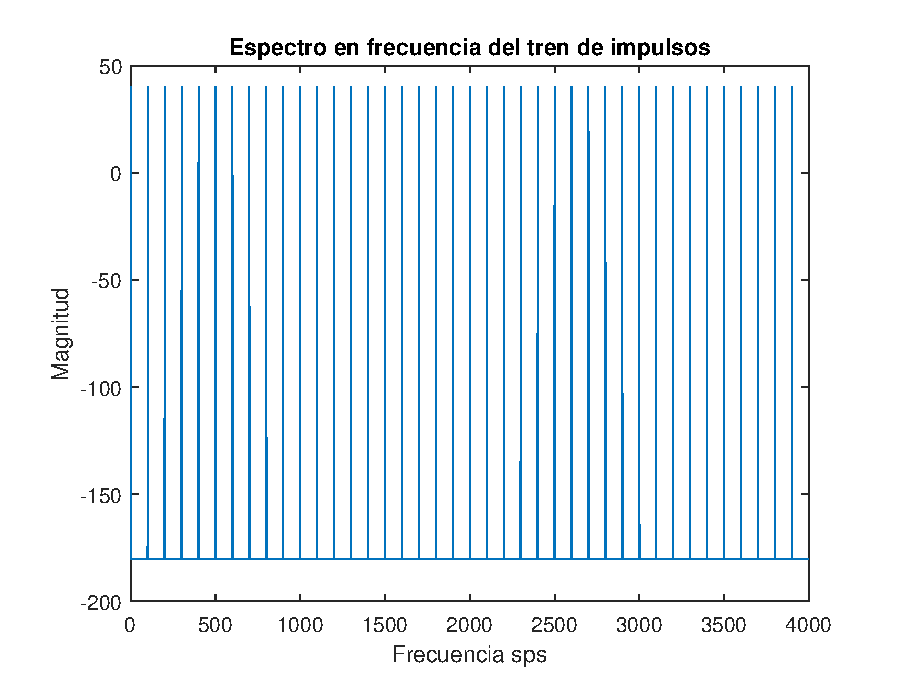
\includegraphics[scale = 0.7]{figures/p1_1frec_tren.eps}
    \caption{Espectro del tren de impulsos generada con la función \textit{exciteV}}
    \label{frec_tren}
\end{figure}

\subsection{Diseño de filtros AR óptimos usando $y = lpc(x,p)$}

Para esta parte se utilizó el código \texttt{p1\_2.m}, adjunto a la entrega.

La sección de código donde se diseñan los filtros que simulan el comportamiento del tracto vocal para cada vocal se muestra a continuación:
\begin{lstlisting}[language = octave]
load vowels

% Diseno de filtros
a_vowel_a = lpc(vowel_a,P);
a_vowel_e = lpc(vowel_e,P);
a_vowel_i = lpc(vowel_i,P);
a_vowel_o = lpc(vowel_o,P);
a_vowel_u = lpc(vowel_u,P);
\end{lstlisting}
donde $P = 15$, el cual corresponde al orden del filtro que se desea generar.

Las respuestas en frecuencia de cada vocal se muestran en las figuras \ref{fig:p1_2a} - \ref{fig:p1_2u}, donde además se destaca el primer y segundo formante.

\begin{figure}[H]
    \centering
    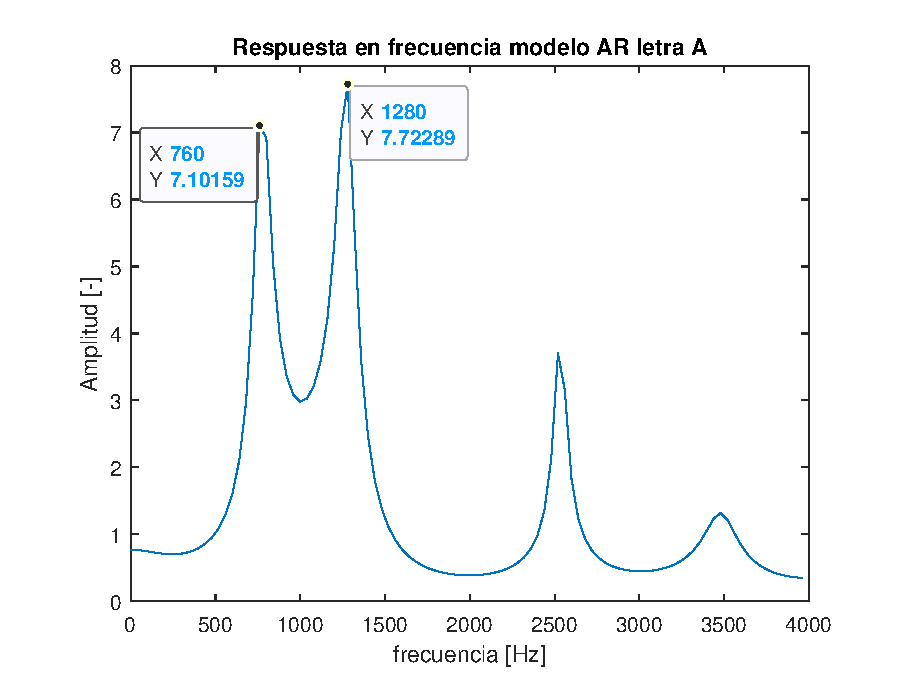
\includegraphics[width = .8\linewidth]{figures/p1_2a.eps}
    \caption{Respuesta en frecuencia de filtro estimado para simular tracto vocal haciendo letra a. Se destaca el primer y segundo formante encontrado.}
    \label{fig:p1_2a}
\end{figure}

\begin{figure}[H]
    \centering
    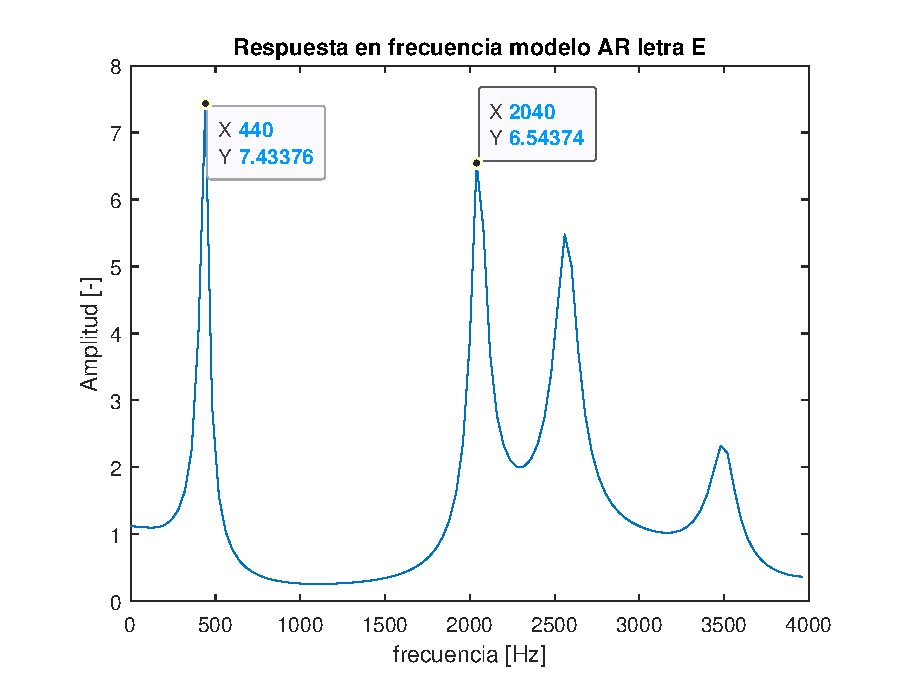
\includegraphics[width = .8\linewidth]{figures/p1_2e.eps}
    \caption{Respuesta en frecuencia de filtro estimado para simular tracto vocal haciendo letra e. Se destaca el primer y segundo formante encontrado.}
    \label{fig:p1_2e}
\end{figure}

\begin{figure}[H]
    \centering
    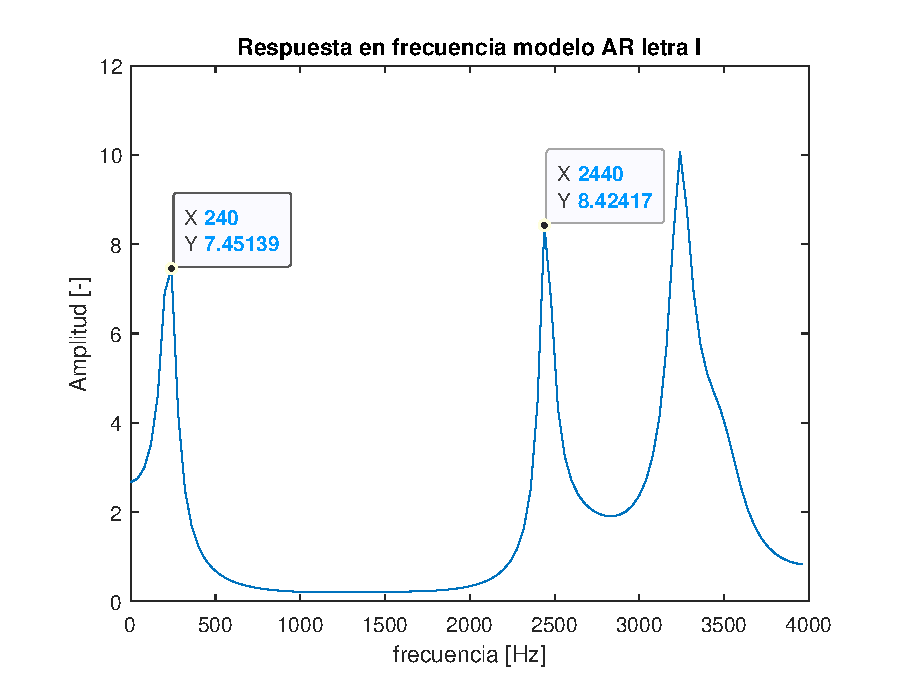
\includegraphics[width = .8\linewidth]{figures/p1_2i.eps}
    \caption{Respuesta en frecuencia de filtro estimado para simular tracto vocal haciendo letra i. Se destaca el primer y segundo formante encontrado.}
    \label{fig:p1_2i}
\end{figure}

\begin{figure}[H]
    \centering
    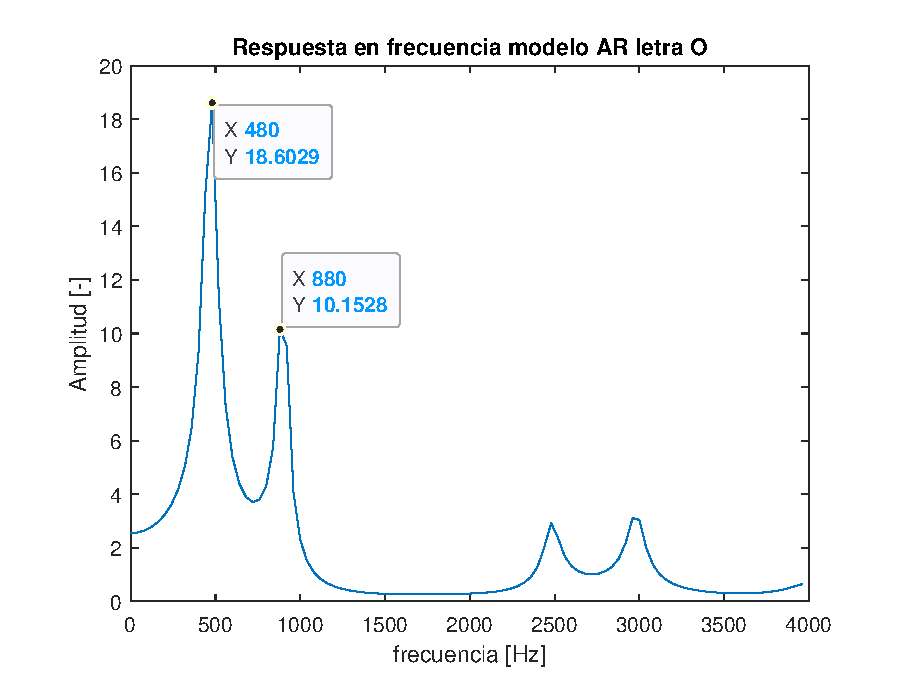
\includegraphics[width = .8\linewidth]{figures/p1_2o.eps}
    \caption{Respuesta en frecuencia de filtro estimado para simular tracto vocal haciendo letra o. Se destaca el primer y segundo formante encontrado.}
    \label{fig:p1_2o}
\end{figure}

\begin{figure}[H]
    \centering
    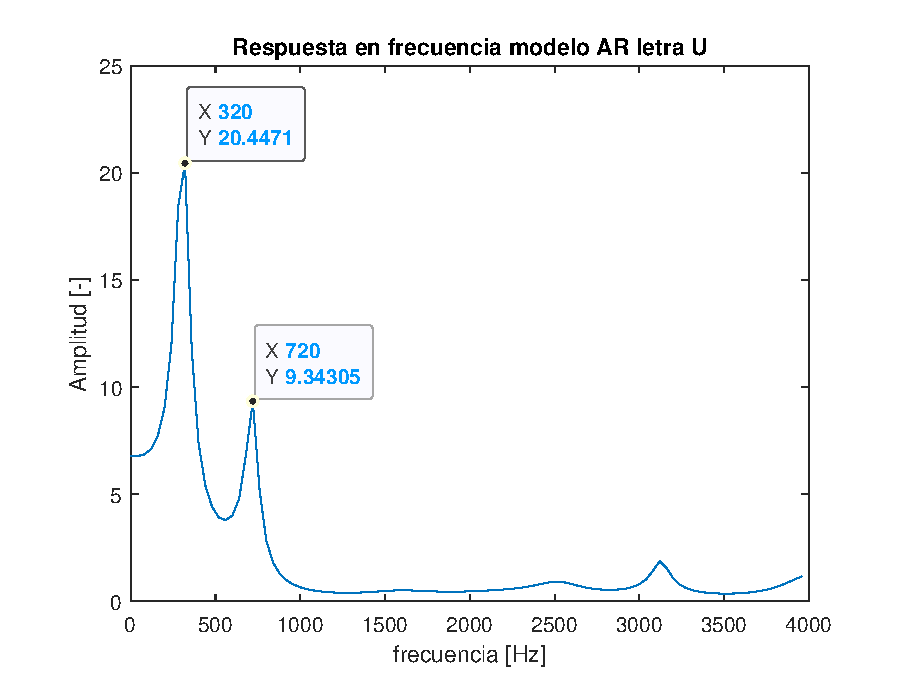
\includegraphics[width = .8\linewidth]{figures/p1_2u.eps}
    \caption{Respuesta en frecuencia de filtro estimado para simular tracto vocal haciendo letra u. Se destaca el primer y segundo formante encontrado.}
    \label{fig:p1_2u}
\end{figure}

De las figuras de las respuestas en frecuencia del tracto vocal por cada vocal se aprecia que los formantes de cada vocal están donde corresponden según el gráfico de formantes mostrado en la figura \ref{fig:p1_formantes}. Por otro lado en algunas vocales se aprecia un menor número de peaks, por lo que un valor menor de $P$ dependiendo la vocal podría ser suficiente (vocales i y u).

\begin{figure}[H]
    \centering
    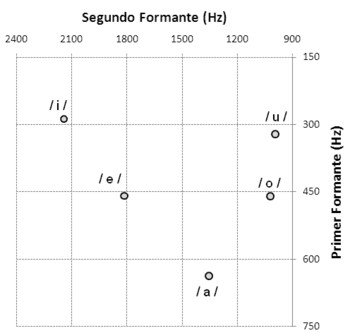
\includegraphics[width = .5\linewidth]{figures/350px-Spanish_Vowel_Formants_Bradlow1995.png}
    \caption{Gráfico de formantes de vocales en habla hispana.}
    \label{fig:p1_formantes}
\end{figure}

\subsection{Uso de filtros diseñados para síntesis de vocales}
Para esta sección se utiliza el código \texttt{p1\_3.m}, el cual se adjunta a la entrega.

Se utilizan los filtros AR diseñados en el punto anterior junto a la señal de tren impulsos generada en el parte 1.1 como entrada a los filtros para sintetizar archivos de audio.

La sección de código donde se genera la señal discreta que imita a un muestreo de una señal de audio de cada vocal se muestra a continuación:

\begin{lstlisting}
%%% 3. Generacion de archivos de audio (filtrado)
y_a = filter(1, a_vowel_a, x);
y_e = filter(1, a_vowel_e, x);
y_i = filter(1, a_vowel_i, x);
y_o = filter(1, a_vowel_o, x);
y_u = filter(1, a_vowel_u, x);
\end{lstlisting}

Con respecto a los archivos de audio generados, si es posible distinguir que vocal corresponde a cada una. Sobre la calidad de audio, todos los sonidos tienen un tono ''robótico'', siendo la letra u la que tiene menos calidad, al menos desde el parlante disponible al momento de escucharla. Las vocales se adjunta al informe en el formato \texttt{matlab\_vowel\_x} siendo \texttt{x} la vocal respectiva.

Para mejorar la calidad del audio se podría filtrar la señal generada con el sistema actual por un filtro pasa bajos a diseñar mediante algún criterio. Lo anterior se plantea debido a que se pueden percibir frecuencias altas en el audio que no son naturales en la voz humana a esa potencia. 

Los gráficos de los espectros en frecuencia de cada vocal sintetizada se muestran en las figuras \ref{fig:p1_3a} - \ref{fig:p1_3u}. Con respecto a las formas obtenidas, como era de esperarse, corresponden a un tren de impulsos con envolvente la respuesta en frecuencia del filtro de la vocal respectiva.

\begin{figure}[H]
    \centering
    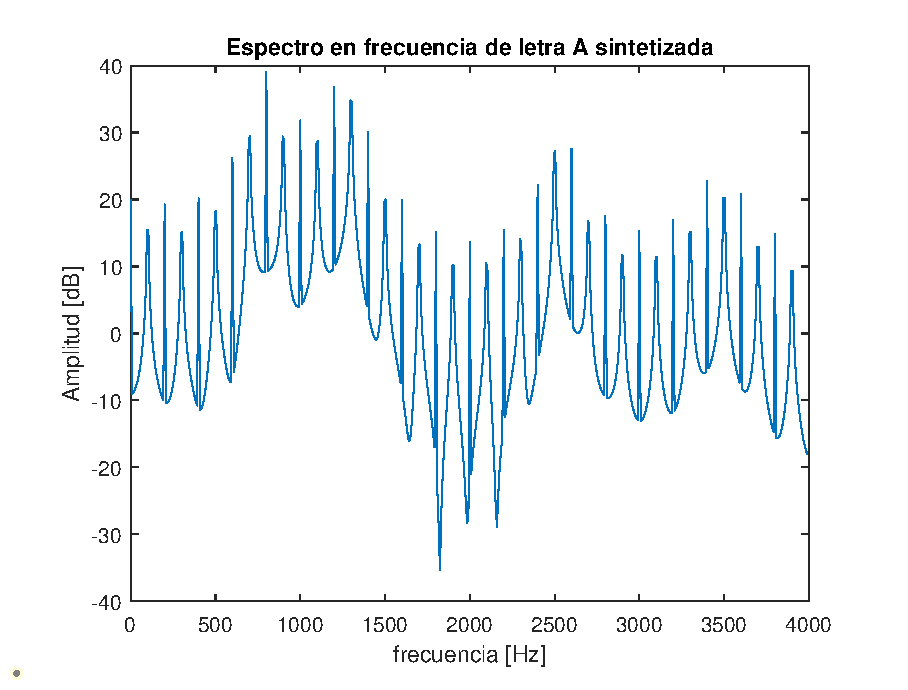
\includegraphics[width = .8\linewidth]{figures/p1_3a.eps}
    \caption{Espectro en frecuencia de letra A sintetizada.}
    \label{fig:p1_3a}
\end{figure}

\begin{figure}[H]
    \centering
    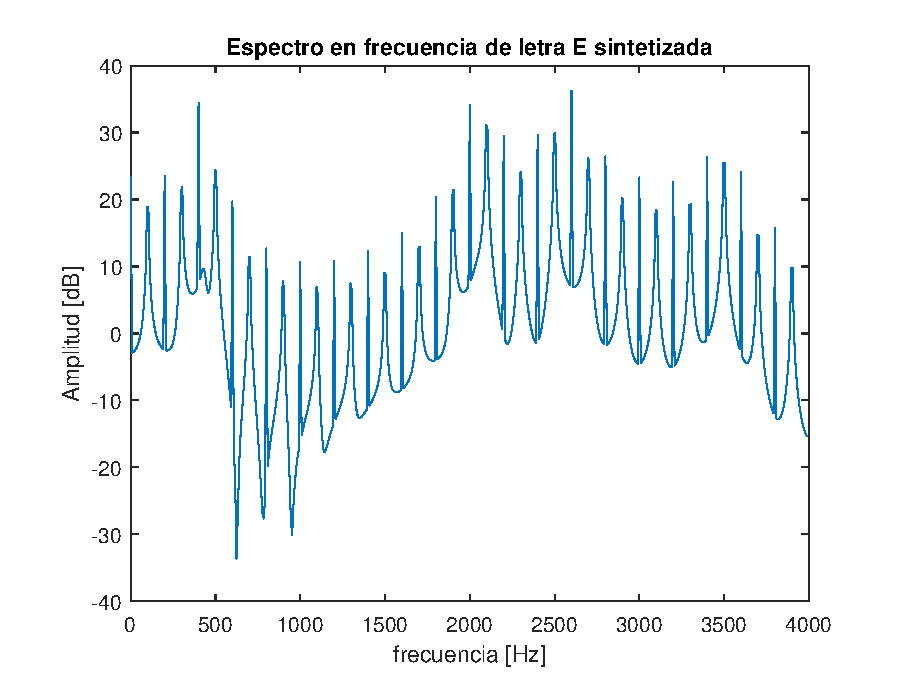
\includegraphics[width = .8\linewidth]{figures/p1_3e.eps}
    \caption{Espectro en frecuencia de letra E sintetizada.}
    \label{fig:p1_3e}
\end{figure}

\begin{figure}[H]
    \centering
    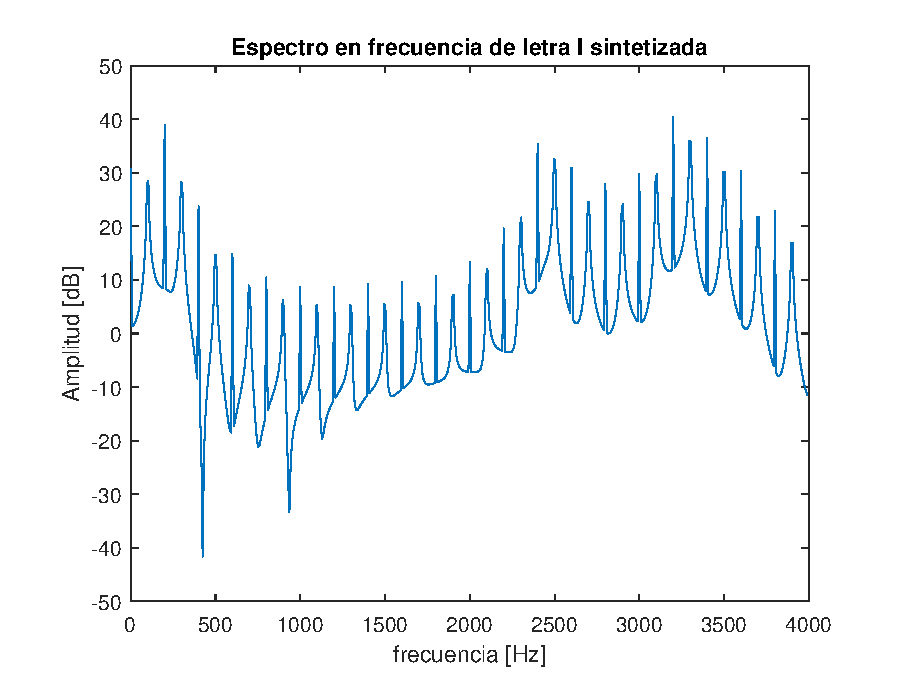
\includegraphics[width = .8\linewidth]{figures/p1_3i.eps}
    \caption{Espectro en frecuencia de letra I sintetizada.}
    \label{fig:p1_3i}
\end{figure}

\begin{figure}[H]
    \centering
    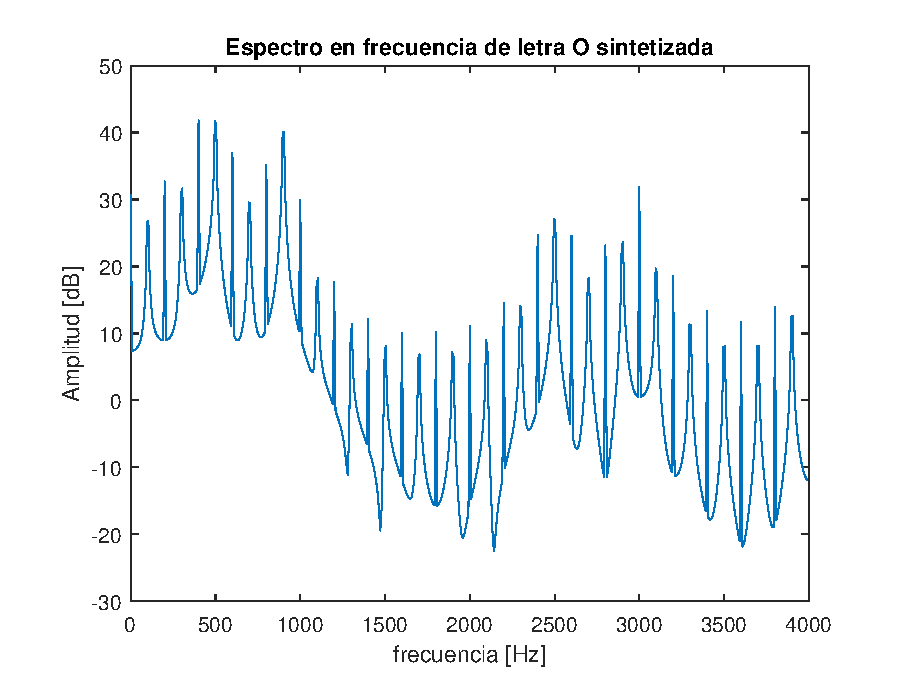
\includegraphics[width = .8\linewidth]{figures/p1_3o.eps}
    \caption{Espectro en frecuencia de letra O sintetizada.}
    \label{fig:p1_3o}
\end{figure}

\begin{figure}[H]
    \centering
    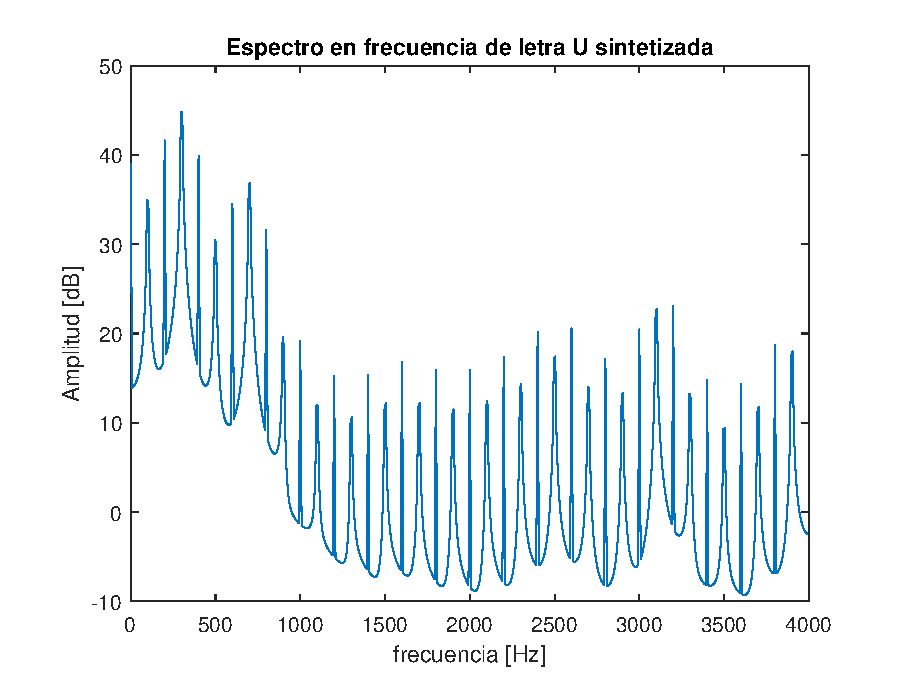
\includegraphics[width = .8\linewidth]{figures/p1_3u.eps}
    \caption{Espectro en frecuencia de letra U sintetizada.}
    \label{fig:p1_3u}
\end{figure}

\subsection{Generación de función $y = mylpc(x,p)$ y comparación con puntos anteriores}

En primer lugar se escribe la función $y=mylpc(x,p)$ la cual corresponde a una implementación del comando $lpc(x,p)$ usado anteriormente. El código se muestra a continuación:
\begin{lstlisting}[language = octave]
function y = mylpc(x,p)
    rx = xcorr(x);    
    rx_toeplitz  = rx(length(x):length(x)+p-1);
    rx = rx(length(x)+1:length(x)+p);

    Ra = toeplitz(rx_toeplitz);

    a = (Ra\rx)';
    y = [1 -a];
end
\end{lstlisting}

donde, obteniendo $R_x$ y $r_x$ a partir de estimaciones de la autocorrelación se resuelve $R_xa = r_x$, para finalmente retornar los parámetros del filtro AR diseñado.

Posteriormente se utiliza la nueva función para repetir los puntos 1.2 y 1.3. Los coeficientes AR obtenidos con el comando $lpc$ y $mylpc$ coinciden para cada vocal. Los gráficos de la respuesta en frecuencia de los filtros diseñados con $mylpc$ se muestran en las figuras \ref{fig:p1_4a} - \ref{fig:p1_4u}, coincidiendo con las obtenidas en 1.2.

Los archivos de audio resultantes se adjuntan a la entrega con el formato \texttt{mylpc\_vowel\_x} siendo \texttt{x} la vocal respectiva.

\begin{figure}[H]
    \centering
    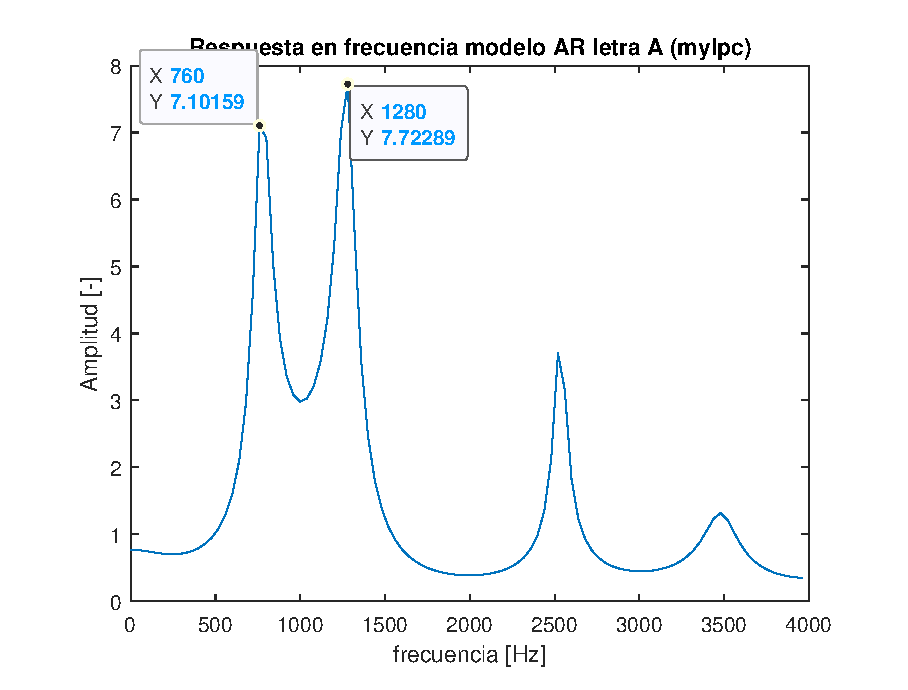
\includegraphics[width = .8\linewidth]{figures/p1_4a.eps}
    \caption{Respuesta en frecuencia de filtro estimado para simular tracto vocal haciendo letra a. Se destaca el primer y segundo formante encontrado ($mylpc$).}
    \label{fig:p1_4a}
\end{figure}

\begin{figure}[H]
    \centering
    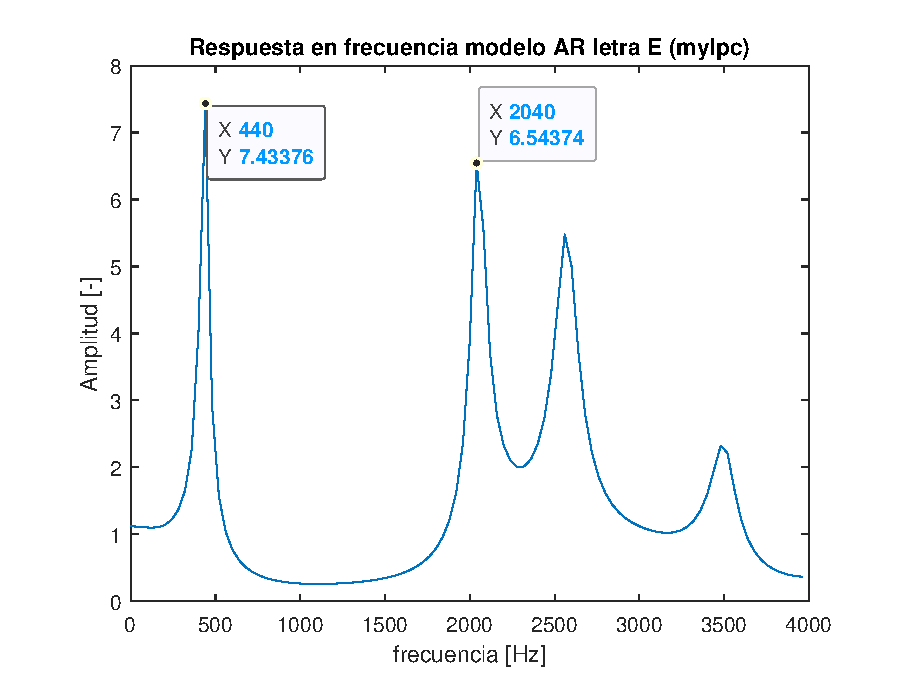
\includegraphics[width = .8\linewidth]{figures/p1_4e.eps}
    \caption{Respuesta en frecuencia de filtro estimado para simular tracto vocal haciendo letra e. Se destaca el primer y segundo formante encontrado ($mylpc$).}
    \label{fig:p1_4e}
\end{figure}

\begin{figure}[H]
    \centering
    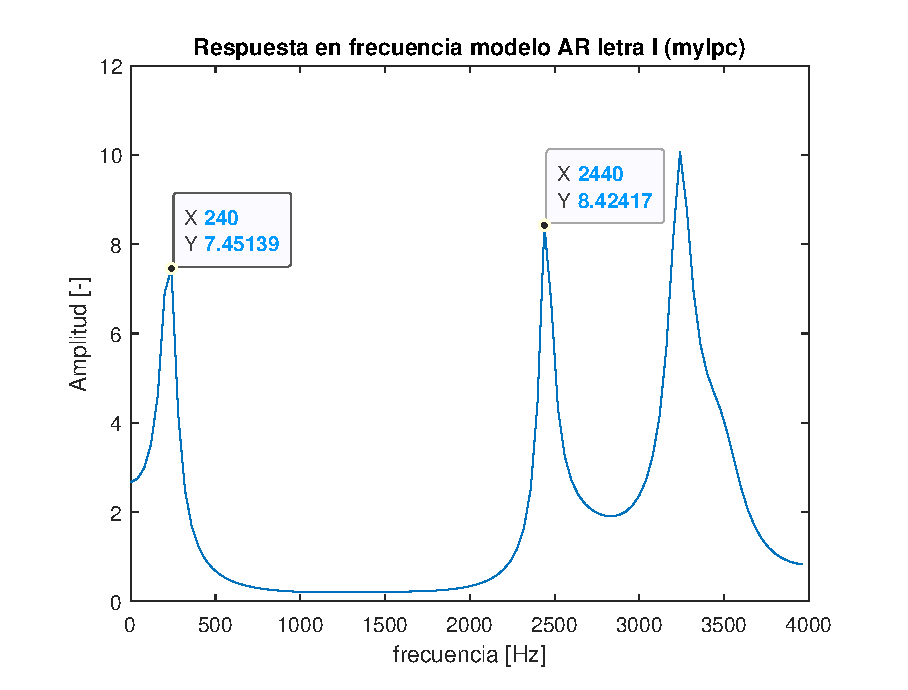
\includegraphics[width = .8\linewidth]{figures/p1_4i.eps}
    \caption{Respuesta en frecuencia de filtro estimado para simular tracto vocal haciendo letra i. Se destaca el primer y segundo formante encontrado ($mylpc$).}
    \label{fig:p1_4i}
\end{figure}

\begin{figure}[H]
    \centering
    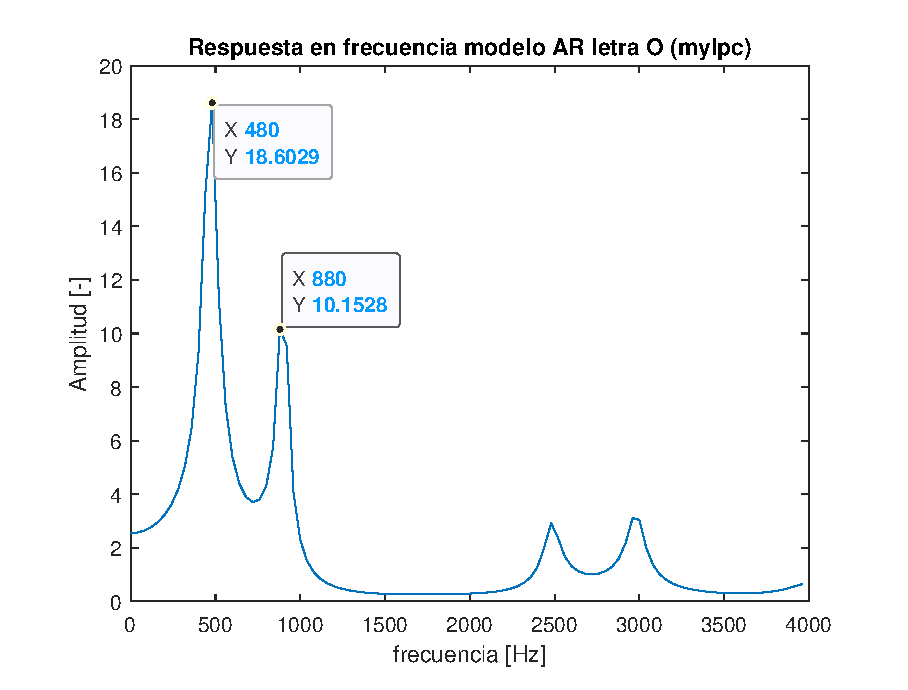
\includegraphics[width = .8\linewidth]{figures/p1_4o.eps}
    \caption{Respuesta en frecuencia de filtro estimado para simular tracto vocal haciendo letra o. Se destaca el primer y segundo formante encontrado ($mylpc$).}
    \label{fig:p1_4o}
\end{figure}

\begin{figure}[H]
    \centering
    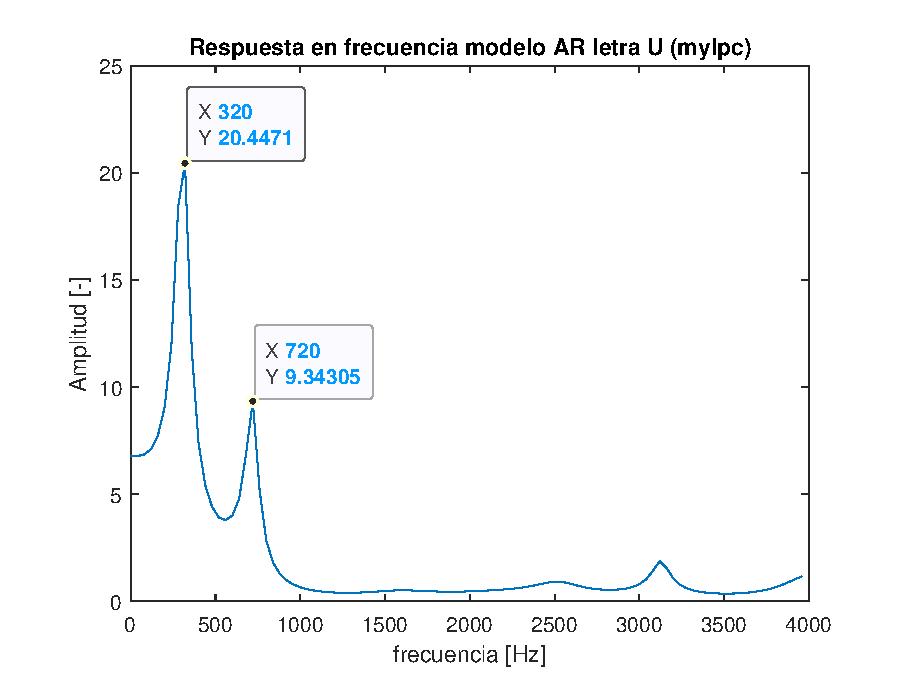
\includegraphics[width = .8\linewidth]{figures/p1_4u.eps}
    \caption{Respuesta en frecuencia de filtro estimado para simular tracto vocal haciendo letra u. Se destaca el primer y segundo formante encontrado ($mylpc$).}
    \label{fig:p1_4u}
\end{figure}




